\chapter{Wideband Channel Measurement}
\section{Scenario}
Modern wireless channels have many characteristics, namely time variance, frequency selectivity, time dispersion, frequency dispersion etc. In the last experiment of Wireless Digital Communication Lab 1, we will measure these wireless channel characteristics by means of a measurement device called channel sounder, which consists of a transmitter generating and transmitting sounding signal and a receiver receiving and processing the received signals. 

If the system components have ideal characteristics, the characteristics of the wireless channel is equivalent to the "equivalent baseband channel", which is shown in figure \ref{fig:ex5:equi_fig}. However, in real systems this is not necessarily the case.

\begin{figure}[H]
	\begin{center}
		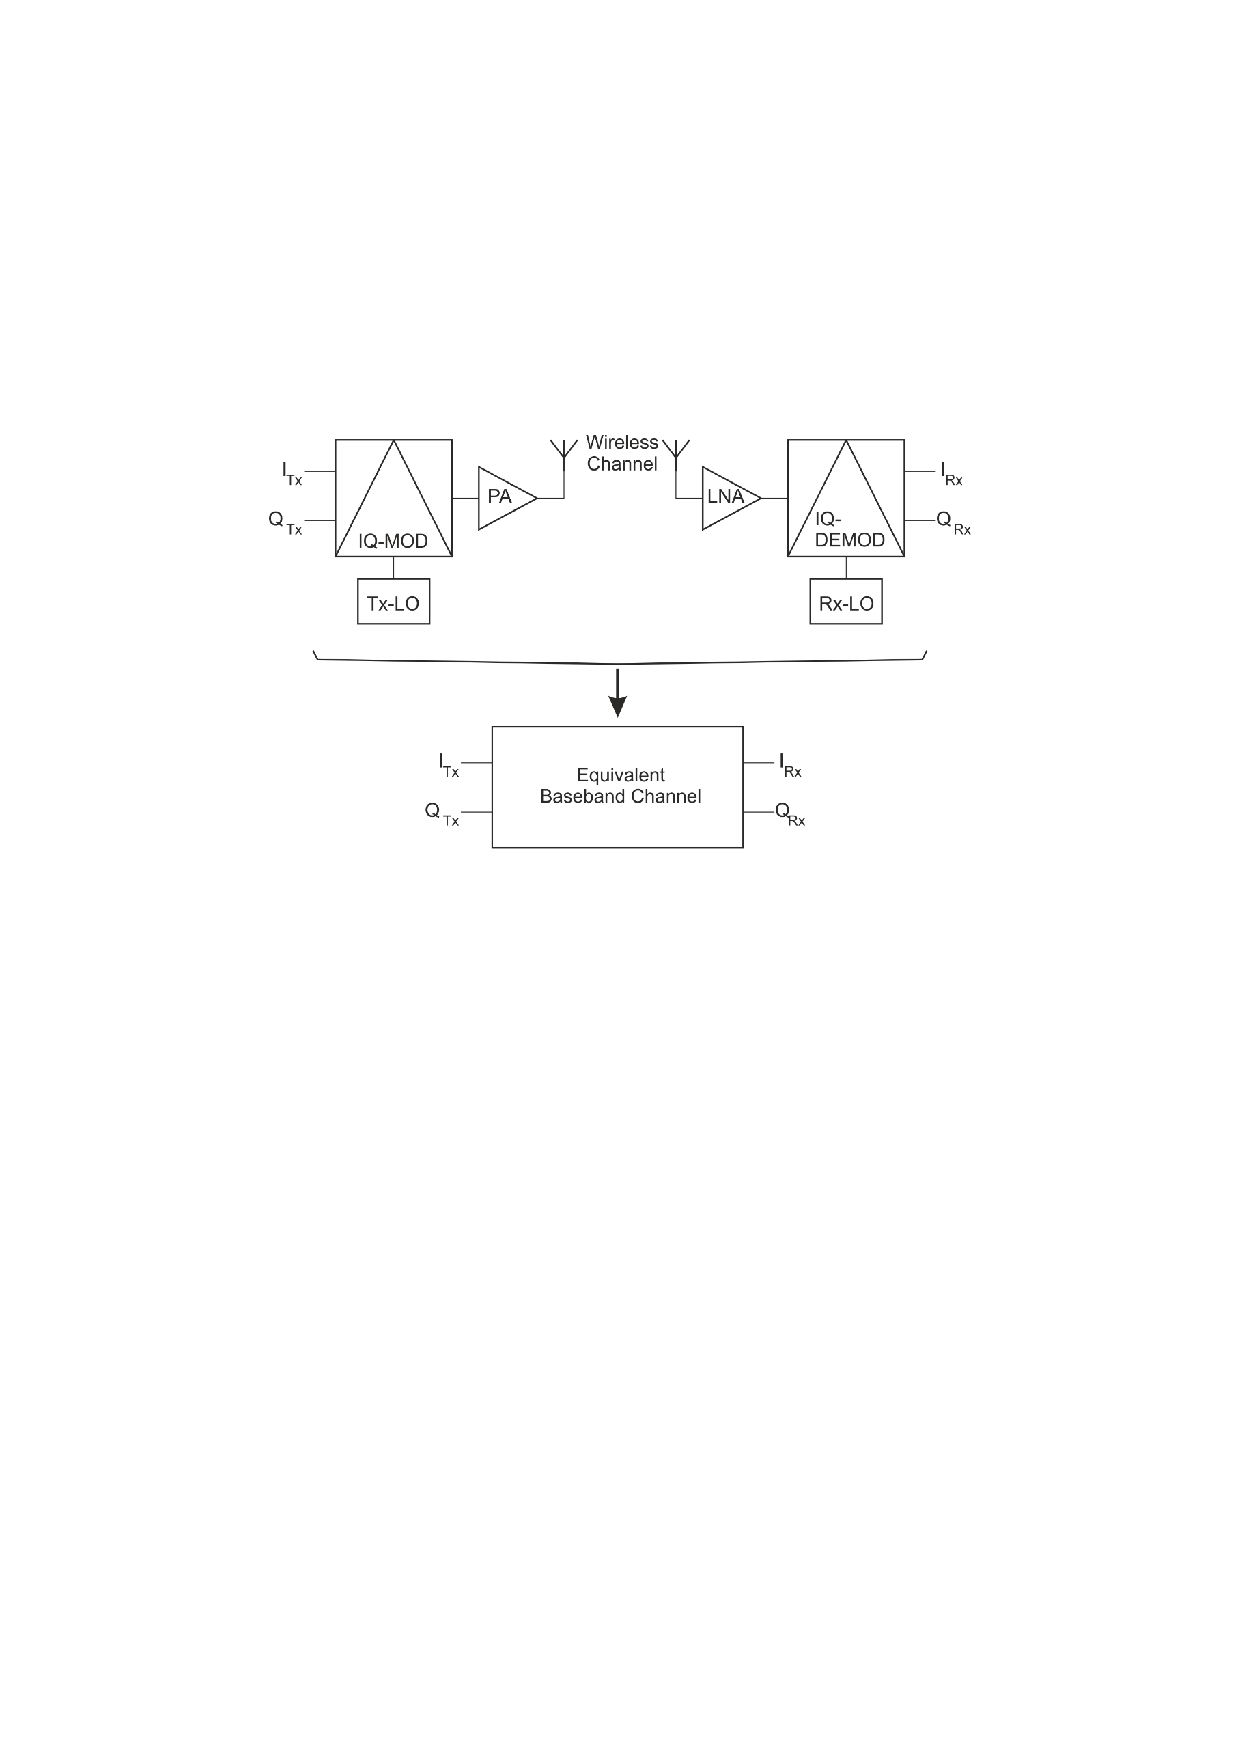
\includegraphics[scale=0.5]{ex5/equivalent_figure.pdf}
		\caption{Equivalent baseband model of the channel measurement \cite{e5}}
		\label{fig:ex5:equi_fig}
	\end{center}
\end{figure}  

Our SDR platform uses wideband mode for the channel measurements. The sampling frequency in this mode is \SI{250}{\mega \hertz}. We transmit signal sequence periodically to have periodic measurements of the wireless channel. The duration of a signal period a sequence of 256 elements (chips); each chip duration is $1/f_{samp} = \SI{4}{\nano \second}$. The total sequence period duration is therefore \SI{1024}{\micro \second}, which has to be larger than the channel excess delay, in our case in the range of \SIrange{0.1}{10}{\micro \second}.

Figure \ref{fig:ex5:derivation} shows the derivation of the measurement concept implementation. The third configuration which shifts the second sequence generator and the correlation function element to the receiver part is appropriate to be implemented, since its input signal comprises of several low energy pulses.

\begin{figure}[H]
	\begin{center}
		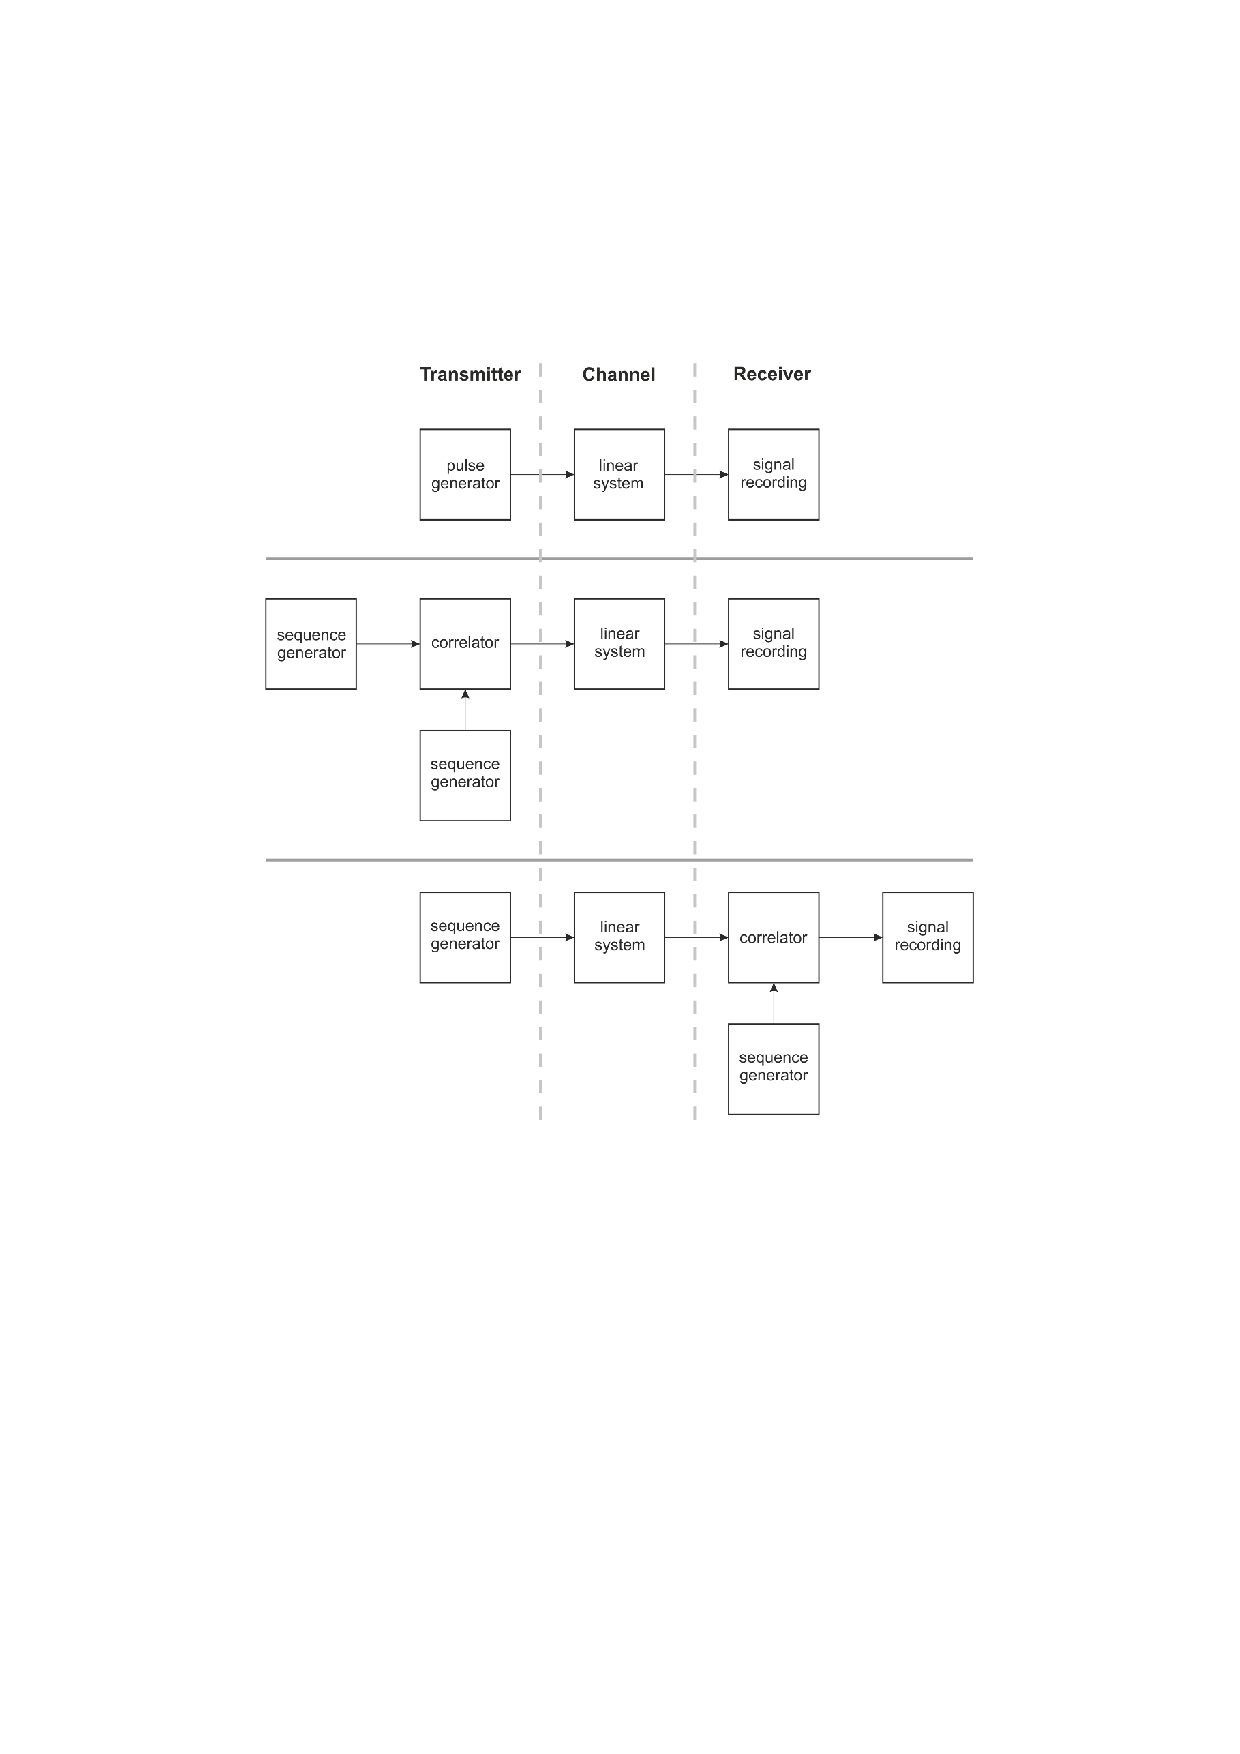
\includegraphics[scale=0.5]{ex5/derivation.pdf}
		\caption{Derivation of the measurement concept implementation \cite{e5}}
		\label{fig:ex5:derivation}
	\end{center}
\end{figure}

Meanwhile the additive measurement noise need to be considered during the signal processing. Averaging signal periods is utilized to increase SNR. The time interval of averaging is termed "snapshot". Regarding the rotation velocity, radius of copper patches and the carrier frequency the maximum Doppler frequency shift is $f_{doppler,max} = f_{carrier}\cdot \frac{v_{max}}{c}=\SI{167}{\hertz}$. The minimal time intervals of the snapshots should be $\frac{1}{2 f_{doppler,max}}=\SI{3}{\milli \second}$.

The time structure of the channel measurements is displayed in Figure \ref{fig:ex5:time_slot}. A certain number of consecutive snapshots composes a measurement "set" and fast time variations of the channel characteristics are included in it. We can calculate the Doppler resolved channel impulse response function from one set, which features the magnitude and the individual Doppler frequency shifts of all multi-path components.

\begin{figure}[H]
	\begin{center}
		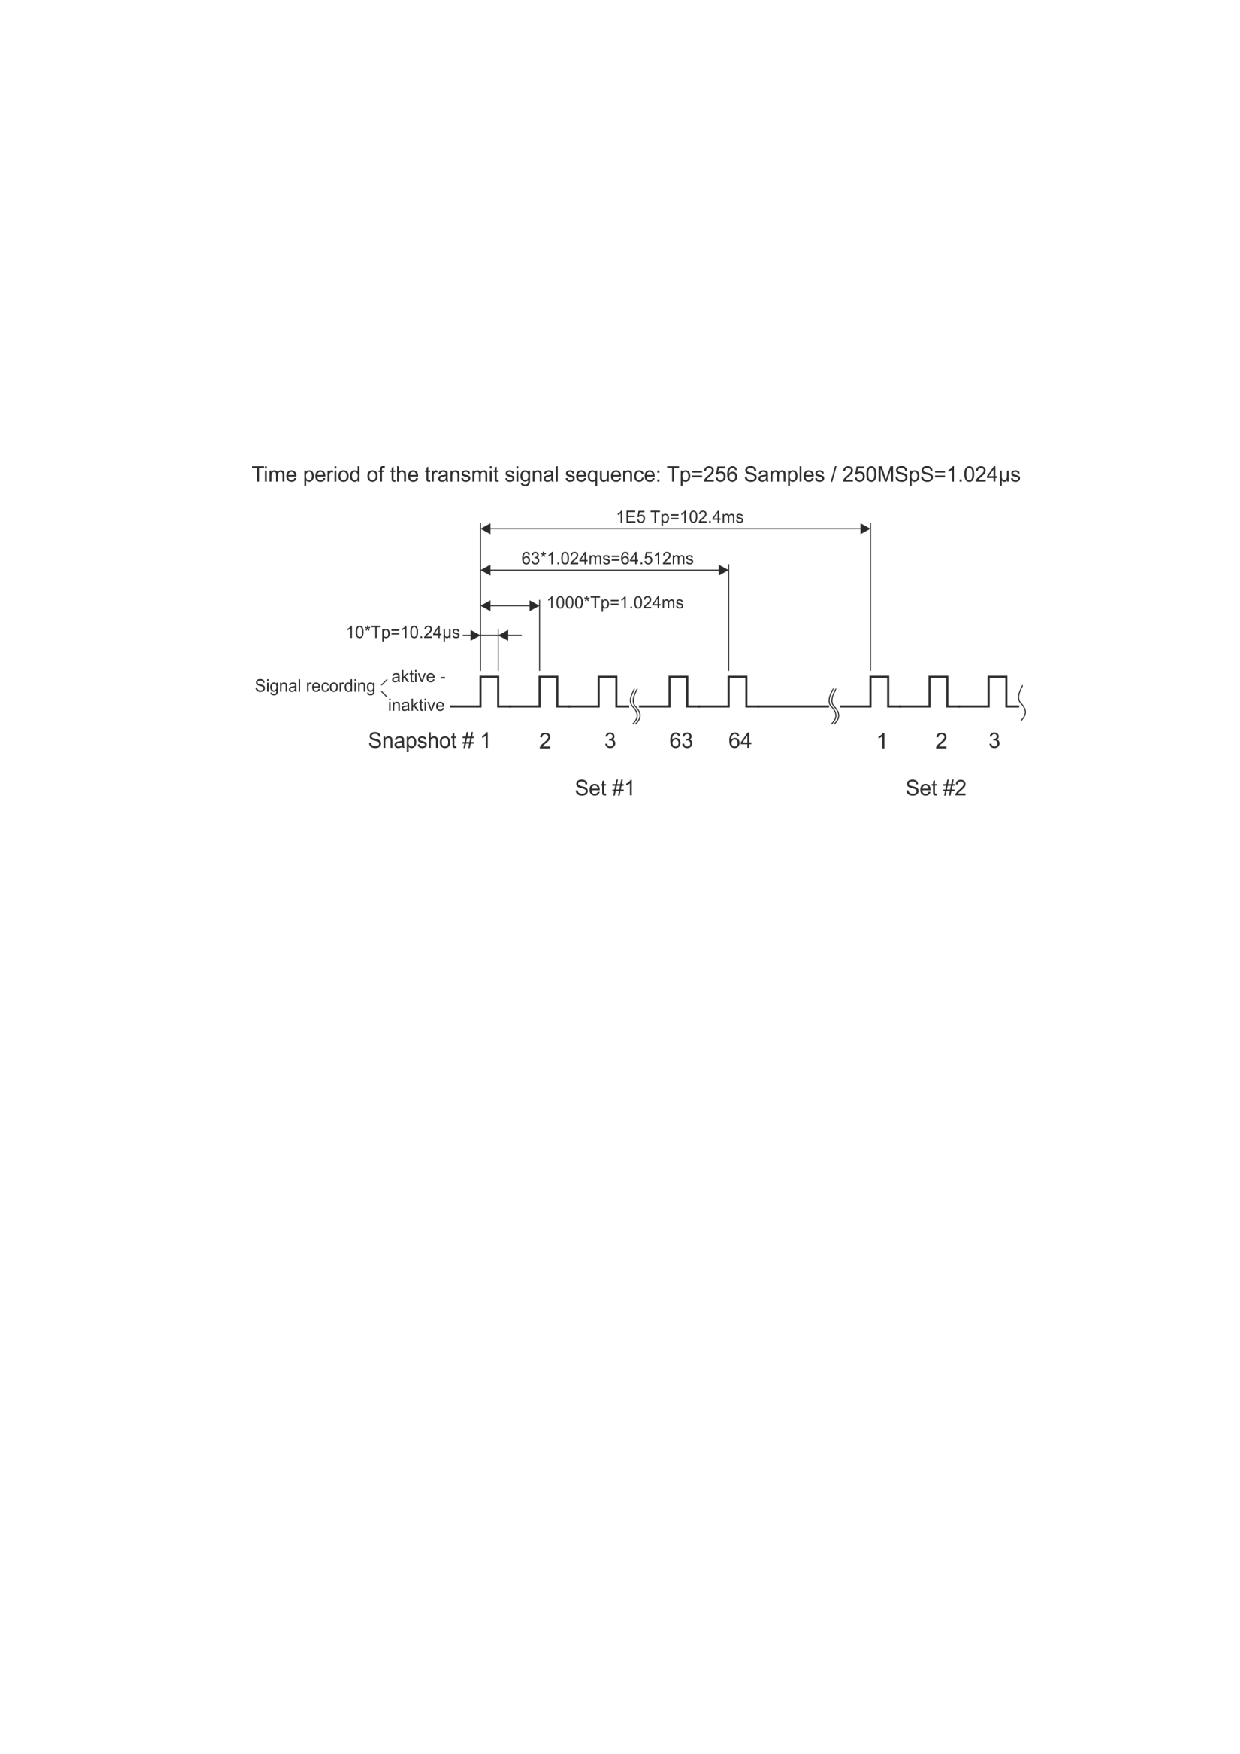
\includegraphics[scale=0.5]{ex5/time_slot.pdf}
		\caption{Time structure of channel measurement \cite{e5}}
		\label{fig:ex5:time_slot}
	\end{center}
\end{figure}

\section{Task}
By means of Matlab script "ChannelSounderTransmission.m" we should process the received signal so as to calculate the channel transfer function, channel impulse response function as well as the Doppler resolved channel impulse response function (on the condition of  rotating disks).
\section{Information about the transmit signal}
\begin{itemize}
	\item Signal name: CHANNELSOUNDER
	\item Parameter specifications: 
\end{itemize}

\begin{figure}[H]
	\begin{center}
		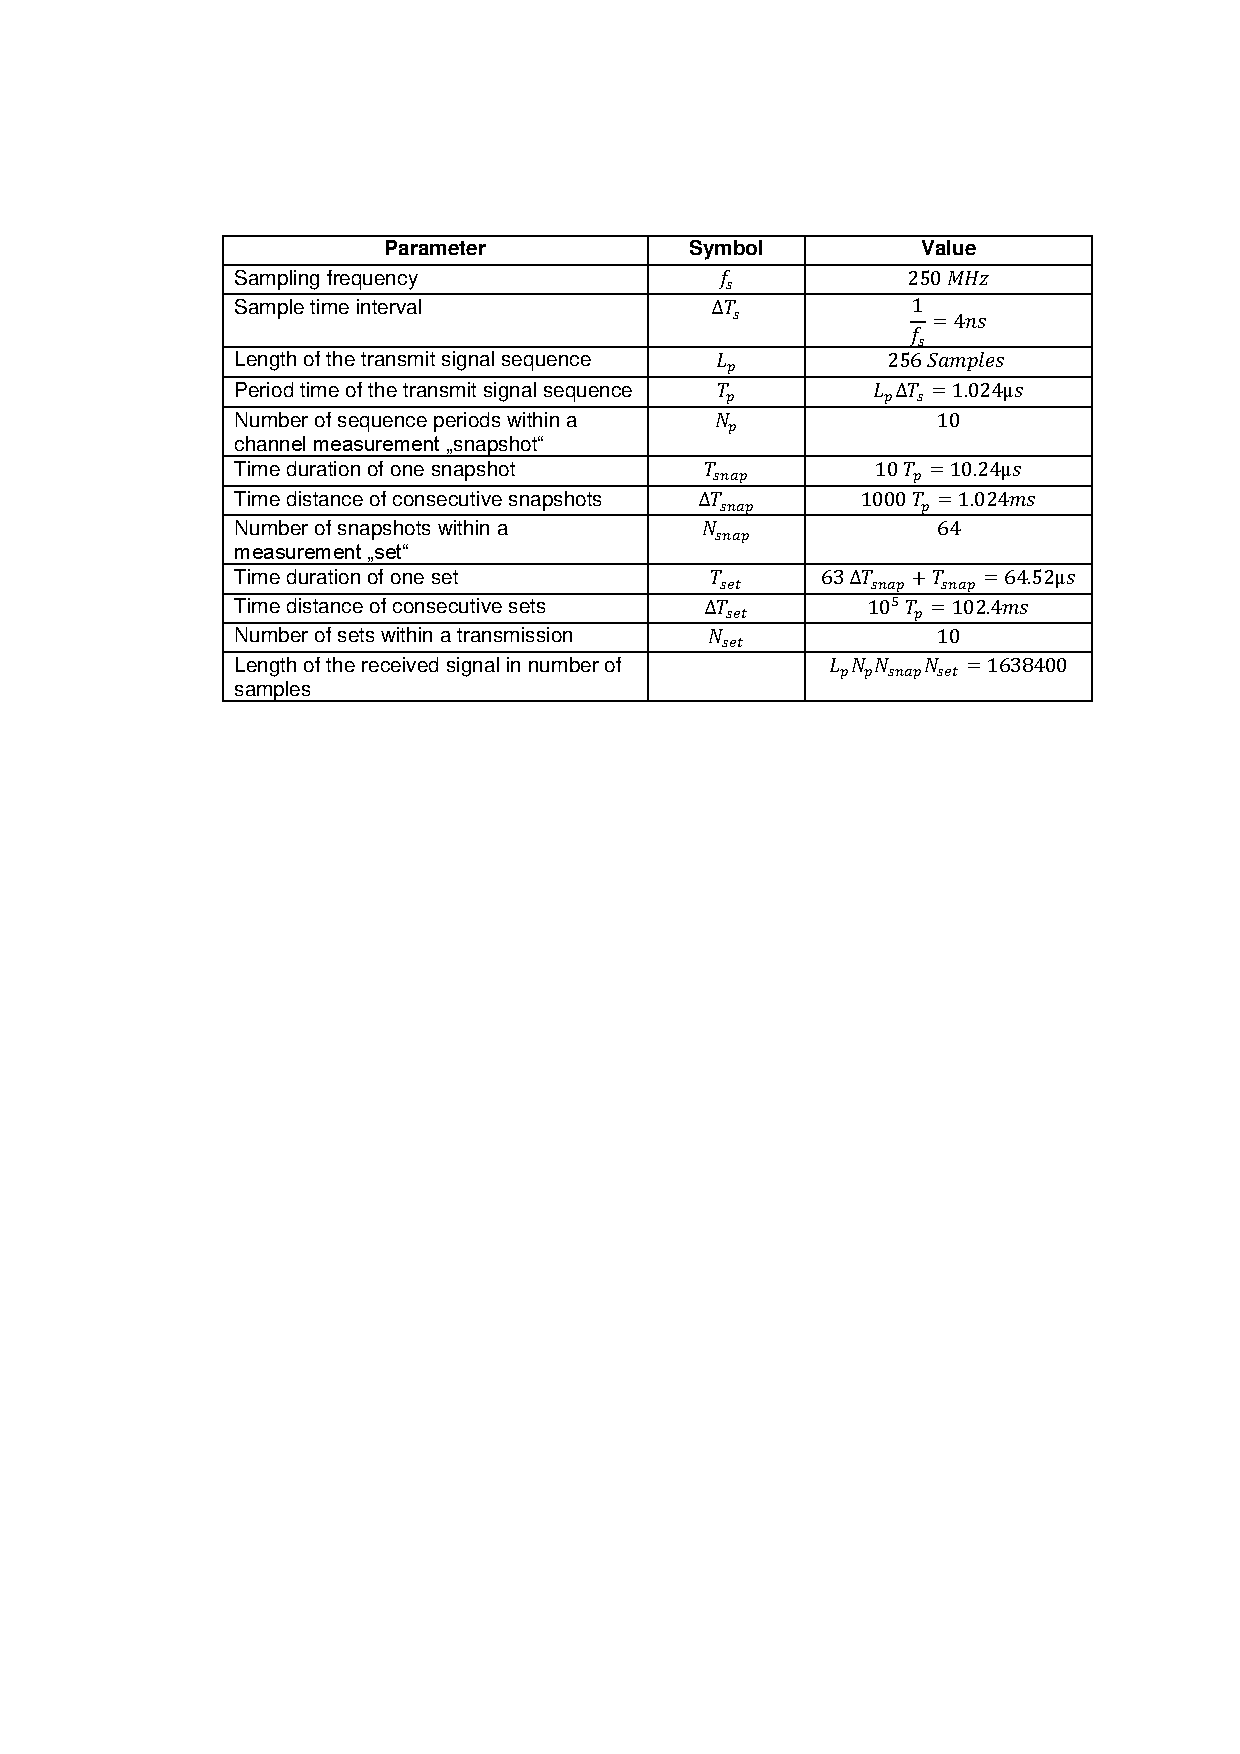
\includegraphics[scale=1]{ex5/parameter.pdf}
		\caption{Parameters of the signal \cite{e5}}
		\label{fig:ex5:parameter}
	\end{center}
\end{figure}



\section{Algorithm description \cite{e5}}
The suggested algorithm is given below:
\begin{enumerate}
	\item Transmit the channel sounding signal with the Matlab script "ChannelSoundertransmission.m". Include the group ID into the local copy of the Matlab script. Select antenna signal x1 for further signal processing.
	\item Reshape the signal vector to a matrix, whose rows is equal to the length of the transmit signal period $L_p = 256$ and the columns is equal to the product $N_p N_{snap} N_{set} = 6400$.
	\item Average every snapshot for SNR enhancement and obtain a single vector of $L_p = 256$ elements for each snapshot.
	\item Perform a FFT in column direction (dimension of delay time)
	\item Calculate the time variant transfer function $H(f,t)$. The transformation result vectors should be divided element wise by the elements of the calibration vector $Y_{cal}$ (in our case $Y1_{cal}$). Since the SDR system cannot transfer the DC component (frequency $\SI{0}{\hertz}$), the value of the transfer function at this point should be replaced by a linear interpolation value:
	$$ H(0,t) = \frac{1}{2} \left( H(-\Delta f,t)+ H(\Delta f,t) \right) $$
	\item Depict the results of the time variant (magnitude) transfer functions by different diagrams for consecutive measurement sets or by Matlab function "surf".
	\item Calculate the time variant impulse response functions. All columns of transformation result should be element wise multiplied by the elements of the "windowed correction vector" $W_{FD}./Y_{cal}$. Its effect is to reduce artificial oscillations (side lobes) in time domain. Instead of using rectangular windowing, in that it produces severe oscillations in the transformation space, we use Gaussian-shape frequency domain window function $W_{FD}$. A time discrete version of the window function $W_{FD}(k)$ should be calculated and it consists of $L_p$ elements and meanwhile be normalized with the mean value 1. The linear interpolation is also required to correct the DC frequency.
	\item Transfer the result to time domain and plot the result as step 6.
	\item Calculate the Doppler resolved channel response functions. The time variant impulse response function should be windowed in observation domain by Gaussian window function:
	$$ W_{TD}(t) = \exp \left( - \left( \frac{t-T_{set}/2}{t_g} \right)^2 \right) $$.
	The cutoff frequency should be chosen to be $t_g \approx 15 \Delta T_{snap}$. A time discrete and normalized version of the window function should be calculated:
	$$ W_{TD} (n) = \frac{W_{TD}(n)}{\frac{1}{N_{snap}} \Sigma W_{TD} (n)} $$
	\item Perform a FFT transformation with respect to observation time - not delay time. Divide the transformation output the number of snapshots per set $N_{snap}$ so that the magnitude level of the multipath contributions here are the same as in the time variant impulse response function.
	\item Depict the Doppler resolved channel impulse response functions by Matlab function: "surf"
\end{enumerate}
\section{Observation and interpretation}
After implementing the algorithm mentioned above we depict the results shown as follows.
\begin{figure}[H]
	\begin{center}
		\subfigure[]{\label{fig:ex5:CIR}
			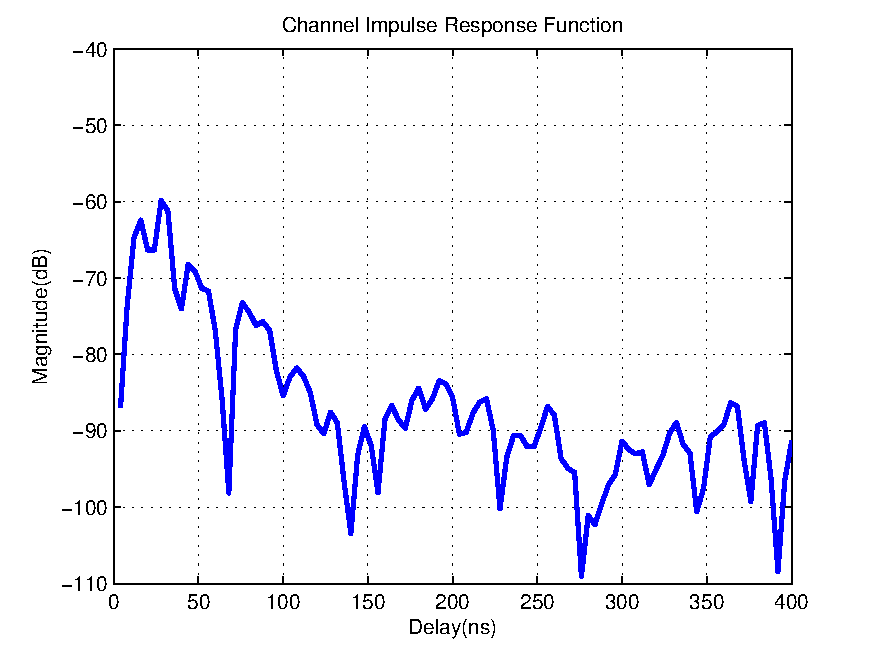
\includegraphics[width=4in]{ex5/channel_impulse_response.pdf} }
		\hspace{1in} %\vspace{x mm}
		\subfigure[]{\label{fig:ex5:channel transfer function}
			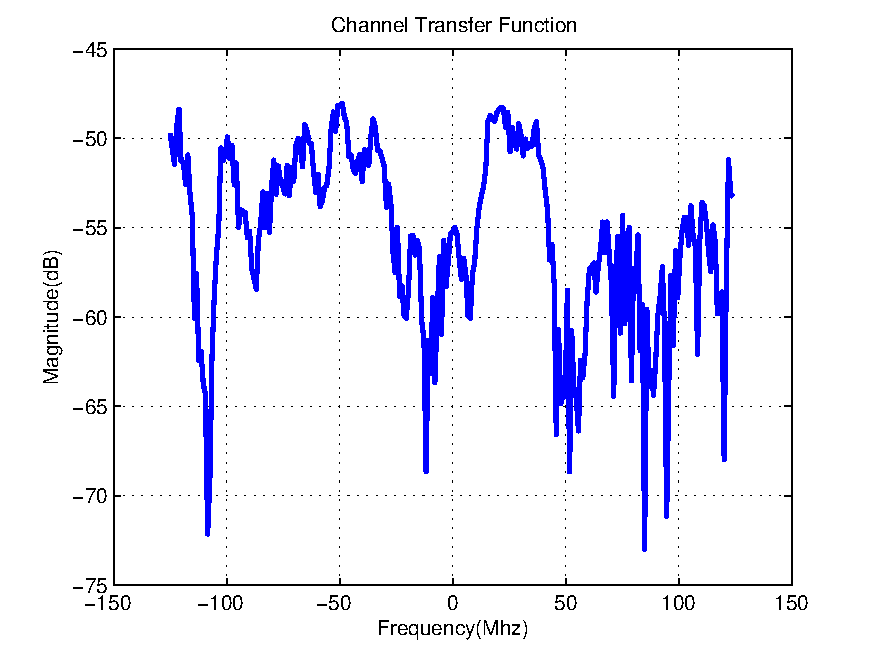
\includegraphics[width=4in]{ex5/channel_transfer_function.pdf} }
	\end{center}
	\caption{Measured channel impulse response function \ref{fig:ex5:CIR} and measured channel transfer function \ref{fig:ex5:channel transfer function}}
	\label{fig:CIR and CTF}
\end{figure}

\begin{figure}[H]
	\begin{center}
		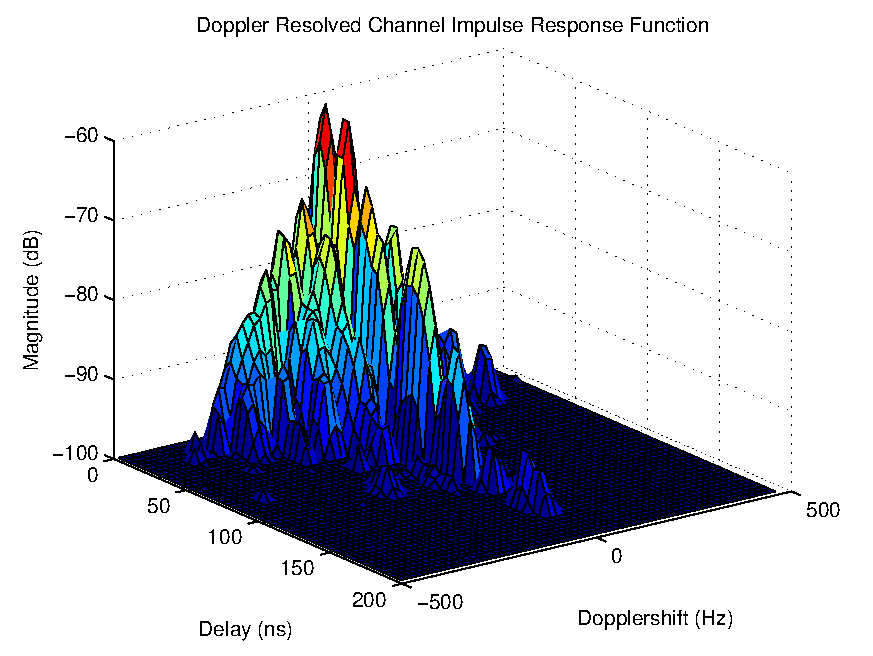
\includegraphics[scale=1]{ex5/doppler_resolved_cirf.pdf}
		\caption{Measured Doppler resolved channel impulse response functions (magnitude), rotating disks}
		\label{fig:ex5:doppler}
	\end{center}
\end{figure}

\section{Summary}
In the experiment we have measured the wireless channel characteristics with the help of channel measurement device channel sounder. Meanwhile we have also calculated and analyzed the relationship like time variant transfer function, channel impulse response and so on. They are calculated by Fourier transform. From the Doppler resolved channel impulse response function we can observe the multipath amplitude as well as the Doppler shift caused by the rotation of the disk. 